\documentclass{article}
\usepackage[utf8]{inputenc}
\usepackage{tikz}
\usepackage{amsmath}
\usetikzlibrary{patterns}
\title{Kinematics}
\author{}
\date{}

\begin{document}

\maketitle

\section{Introduction}
Kinematics is the science of motion that treats the subject without regard to the forces that cause it. Within the science of kinematics, one studies the position, the velocity, the acceleration, and all higher order derivatives of the position variables(with respect to time or any other variable(s)).\\\\
Links and joints are the fundamental components of a robot. \textbf{Joints} represent movement on one rotational axis(x, y or z as rotational axis), or a one parameter translation(motion on x,y, or z axis)(one degree of freedom per joint). To fully represent an object in 3d space, we need six parameters; three for rotation $(\alpha,\beta,\gamma)$ and three for translation($(x,y,z)$-position of joint) (any more is considered redundant), because of this most robots are constructed using six joints to be able to fully express their position and orientation in 3d. \textbf{Links} are the static(unchanging) parts of a robot that connect joints to each other. Given n joints you will have n-1 links; think of links as edges and joints as nodes in a graph.\newpage
\textbf{Examples of joints:}\\
prismatic, spherical, planar(translation with one degree of freedom)\\
revolute, screw, cylindrical(rotational with one degree of freedom)\\
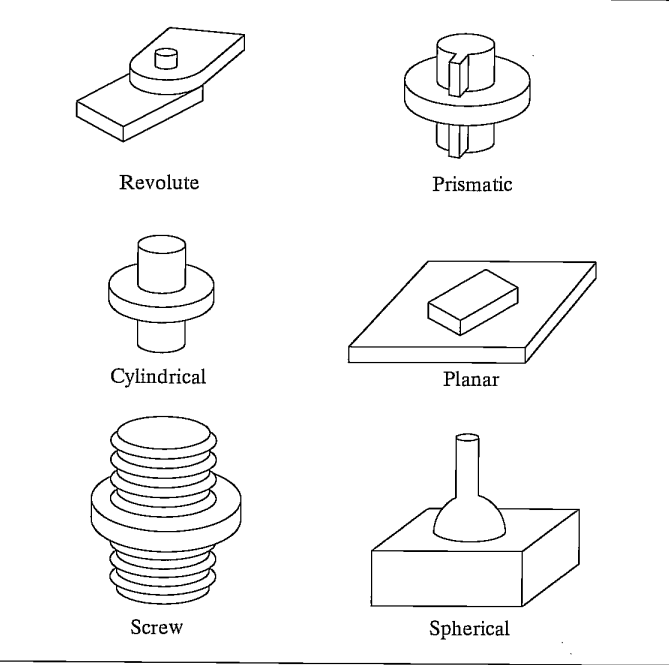
\includegraphics[width=7cm]{type_of_joints.png} \newpage

\section{Conventions for link-frame assignment}
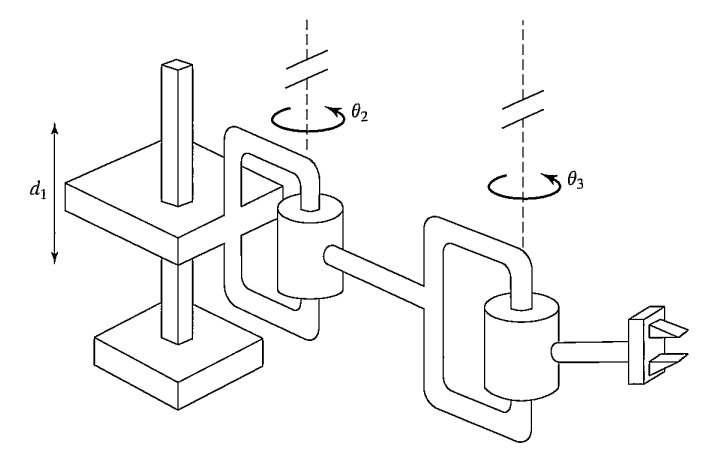
\includegraphics[width=7cm]{PRR.png}\\
\textbf{Algorithm: }\\
\textbf{1.} Identify the joint axes and imagine (or draw) infinite lines along them. For
steps 2 through 5 below, consider two of these neighboring lines (at axes i and
i + 1).\\\\
\textbf{2.} Identify the common perpendicular between them, or point of intersection.
At the point of intersection, or at the point where the common perpendicular
meets the ith axis, assign the link-frame origin.\\
\textbf{3.} Assign the $z_i$ axis pointing along the ith joint axis.\\
\textbf{4.}Assign the $x_i$ axis pointing along the common perpendicular, or, if the axes
intersect, assign $x_i$ to be normal to the plane containing the two axes.\\\\
\textbf{5.} Assign the $y_i$ axis to complete a right-hand coordinate system(optional step).\\\\
\textbf{6.} Assign frame \{0\} to match frame \{1\} when the first joint variable is zero. For {N}, choose an
origin location and $x_n$ direction freely, but generally so as to cause as many
linkage parameters as possible to become zero.\\\\
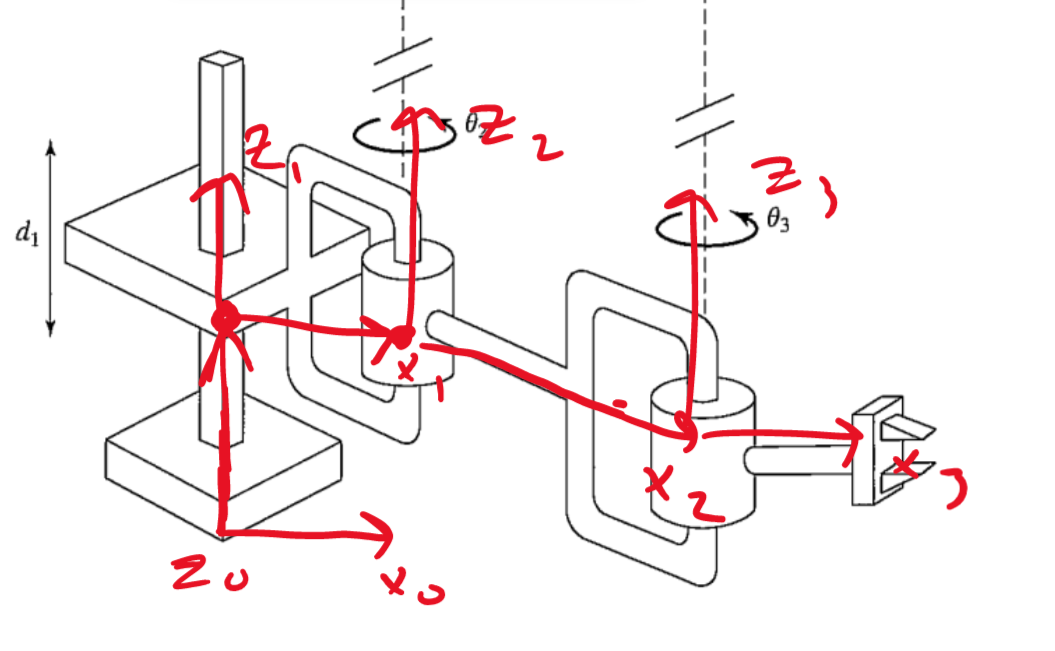
\includegraphics[width=7cm]{PRR_labeled.png}

\section{Parameters for dh table}
The DH table is a method for organizing parameters from a system of known joints, links, and frames. These parameters give us general formulas for constructing the transformations matrices required for computations. \\\\
$a_i$=Distance from $z_{i}$ to $z_{i+1}$ along the $x_i$(this is the link length, and mutual perpendicular between frame \{i\} and \{i+1\})\\\\
$\alpha_i$=link twist angle, angle from $z_{i}$ to $z_{i+1}$ measured along $x_{i}$ (angle between axis i and i+1)\\\\
$d_i$=link offset, the distance from $x_{i-1}$ to $x_{i}$ measured along $z_{i}$ (the offset distance of one link to the next)\\\\
$\theta_i$=the angle from $x_{i-1}$ to $x_{i}$ measured along $z_{i}$ (rotation of link w.r.t. its neighbor along common axis)\\\\

\begin{tabular}{ |p{3cm}|p{3cm}|p{3cm}| p{3cm} | p{3cm} |}
\hline
\multicolumn{5}{|c|}{DH table} \\
\hline
Frame \{i\} & \textbf{$a_{i-1}$} & \textbf{$\alpha_{i-1}$} & \textbf{$d_i$} & \textbf{$\theta_i$} \\
\hline
\textbf{1} & 0     & 0 & $d_1$ & $\theta_1=0$\\
\textbf{2} & $L_1$ & 0 & 0 & $\theta_2$\\
\textbf{3} & $L_2$ & 0 & 0 & $\theta_3$\\
\hline
\end{tabular}\\
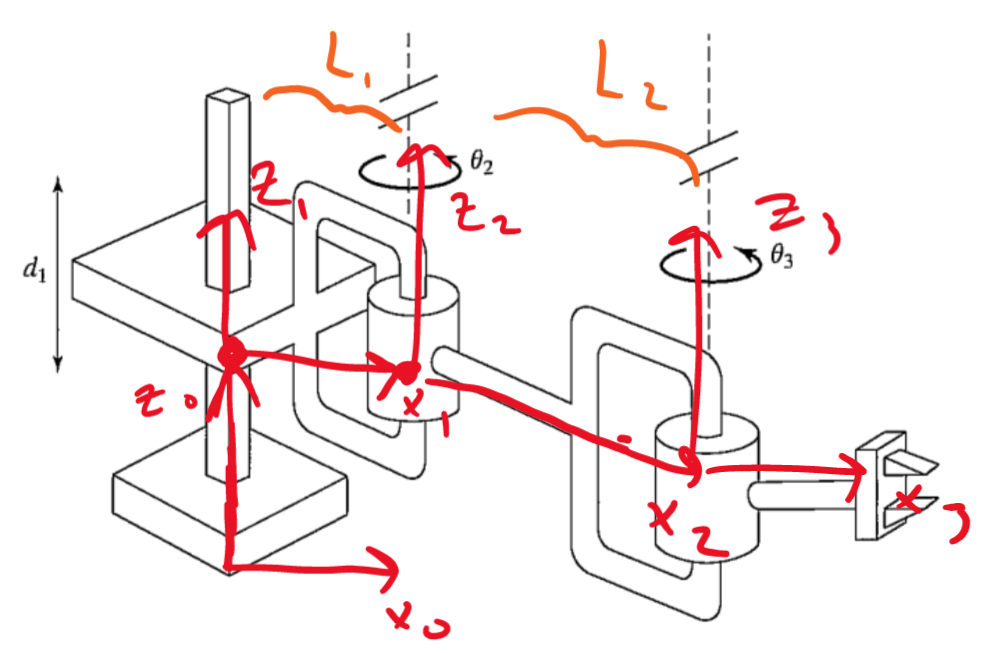
\includegraphics[width=7cm]{PRR_labeled2.png}

\section{dh table to transformation matrix}
Now that we have filled out the DH table, we can make all our transformation matrices using the matrix formula, Note the transformation uses rotation basis: $(R_z(\theta_i)R_x(\alpha_{i-1}))^T$. Tip - Each row corresponds to one transformation matrix, so row 1 has all the variables need for ${}^0_1T$, row 2 has all the variables for ${}^1_2T$ and so on.\\\\
${}^{i-1}_{i}T=\begin{bmatrix}
c\theta_i & -s\theta_i & 0 & a_{i-1}\\
s\theta_ic\alpha_{i-1} & c\theta_ic\alpha_{i-1} & -s\alpha_{i-1} & -s\alpha_{i-1}d_{i}\\
s\theta_is\alpha_{i-1} & c\theta_is\alpha_{i-1} & c\alpha_{i-1} & c\alpha_{i-1}d_{i}\\
                0 & 0 & 0 & 1
\end{bmatrix}$\\\\
\textbf{Note: } Use c0=1 and s0=0 to simplify.\\
${}^{0}_{1}T=
\begin{bmatrix}
c0 & -s0 & 0 & a_0\\
s0c0 & c0c0 & -s0 & -s0d_1\\
s0c0 & s0c0 & c0 & c0d_1\\
0 & 0 & 0 & 1
\end{bmatrix}=
\begin{bmatrix}
1 & 0 & 0 & 0\\
0 & 1 & 0 & 0\\
0 & 0 & 1 & d_1\\
0 & 0 & 0 & 1
\end{bmatrix}$\\\\
${}^{1}_{2}T=
\begin{bmatrix}
c\theta_2 & -s\theta_2 & 0 & L_1\\
s\theta_2c0 & c\theta_2c0 & -s0 & -s0d_2\\
s0c0 & s0c0 & c0 & c0d_2\\
0 & 0 & 0 & 1
\end{bmatrix}=
\begin{bmatrix}
c\theta_2 & -s\theta_2 & 0 & L_1\\
s\theta_2 & c\theta_2 & 0 & 0\\
0 & 0 & 1 & 0\\
0 & 0 & 0 & 1
\end{bmatrix}$\\\\
${}^{2}_{3}T=
\begin{bmatrix}
c\theta_3 & -s\theta_3 & 0 & L_2\\
s\theta_3c0 & c\theta_3c0 & -s0 & -s0d_3\\
s0c0 & s0c0 & c0 & c0d_3\\
0 & 0 & 0 & 1
\end{bmatrix}=
\begin{bmatrix}
c\theta_3 & -s\theta_3 & 0 & L_2\\
s\theta_3 & c\theta_3 & 0 & 0\\
0 & 0 & 1 & 0\\
0 & 0 & 0 & 1
\end{bmatrix}$\\\\
The whole system can be manipulated using the transformation:\\
${}^{0}_{3}T={}^{0}_{1}T{}^{1}_{2}T{}^{2}_{3}T$ \newpage

\section{2nd Example}
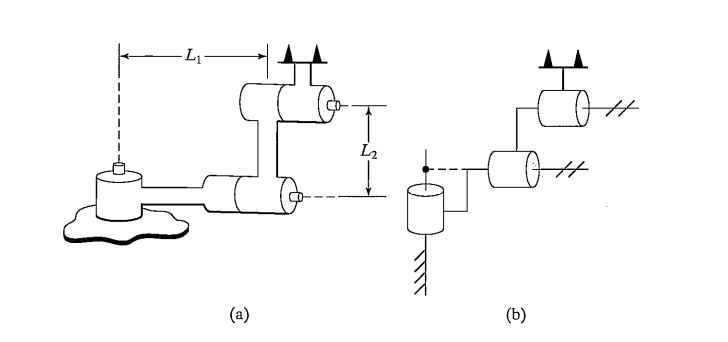
\includegraphics[width=10cm]{RRR_perp.png}\\
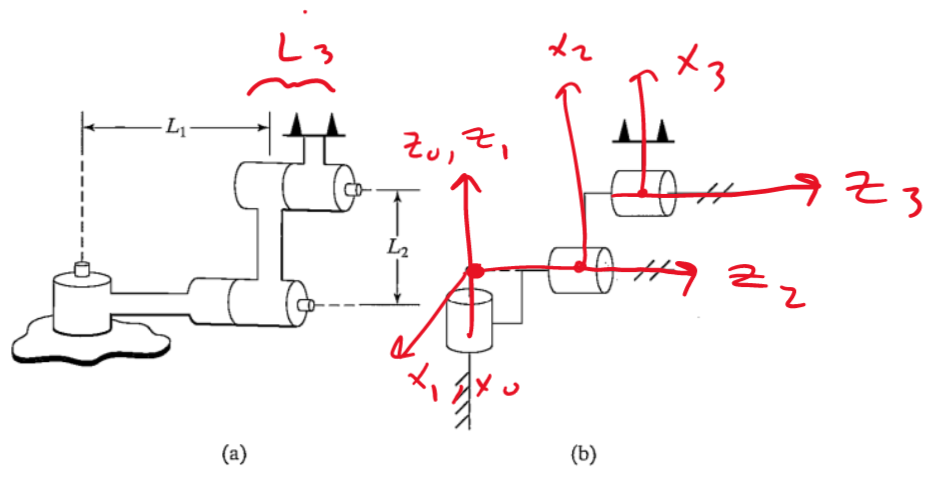
\includegraphics[width=10cm]{RRR_perp_labeled.png}\\\\
$a_0=dist(z_0,z_1) \text{ in } x_0=0\\
a_1=dist(z_1,z_2) \text{ in } x_1=0\\
a_2=dist(z_2,z_3) \text{ in } x_2=L_2\\\\
\alpha_0=angle(z_0,z_1) \text{ in } x_0=0\\
\alpha_1=angle(z_1,z_2) \text{ in } x_1=-90^\circ\\
\alpha_2=angle(z_2,z_3) \text{ in } x_2=0\\\\
d_1=dist(x_0,x_1) \text{ in } z_1=0\\
d_2=dist(x_1,x_2) \text{ in } z_2=L_1\\
d_3=dist(x_2,x_3) \text{ in } z_3=L_3\\\\
\theta_1=angle(x_0,x_1) \text{ in } z_1=\theta_1\\
\theta_2=angle(x_1,x_2) \text{ in } z_2=\theta_2-90^\circ\\
\theta_3=angle(x_2,x_3) \text{ in } z_3=\theta_3$\\\\
\begin{tabular}{ |p{3cm}|p{3cm}|p{3cm}| p{3cm} | p{3cm} |}
\hline
\multicolumn{5}{|c|}{DH table} \\
\hline
Frame \{i\} & \textbf{$a_{i-1}$} & \textbf{$\alpha_{i-1}$} & \textbf{$d_i$} & \textbf{$\theta_i$} \\
\hline
\textbf{1} & 0     & 0 & 0 & $\theta_1$\\
\textbf{2} & 0 & $-90^\circ$ & $L_1$ & $\theta_2-90^\circ$\\
\textbf{3} & $L_2$ & 0 & $L_3$ & $\theta_3$\\
\hline
\end{tabular}\\\\
Using
${}^{i-1}_{i}T=\begin{bmatrix}
c\theta_i & -s\theta_i & 0 & a_{i-1}\\
s\theta_ic\alpha_{i-1} & c\theta_ic\alpha_{i-1} & -s\alpha_{i-1} & -s\alpha_{i-1}d_{i}\\
s\theta_is\alpha_{i-1} & c\theta_is\alpha_{i-1} & c\alpha_{i-1} & c\alpha_{i-1}d_{i}\\
                0 & 0 & 0 & 1
\end{bmatrix}$ we get:\\\\
${}^{0}_{1}T=
\begin{bmatrix}
c\theta_1 & -s\theta_1 & 0 & 0\\
s\theta_1 & c\theta_1 & 0 & 0\\
0 & 0 & 1 & 0\\
0 & 0 & 0 & 1
\end{bmatrix}$\\\\
${}^{1}_{2}T=
\begin{bmatrix}
c(\theta_2-90^\circ) & -s(\theta_2-90^\circ) & 0 & 0\\
0 & 0 & 1 & L_1\\
s(\theta_2-90^\circ) & c(\theta_2-90^\circ) & 0 & 0\\
0 & 0 & 0 & 1
\end{bmatrix}$\\\\
${}^{2}_{3}T=
\begin{bmatrix}
c\theta_3 & -s\theta_3 & 0 & L_2\\
s\theta_3 & c\theta_3 & 0 & 0\\
0 & 0 & 1 & L_3\\
0 & 0 & 0 & 1
\end{bmatrix}$\\\\


%\pagestyle{empty}

% Note. This illustration was originally made with PSTricks. Conversion to
% PGF/TikZ was straightforward. However, I could probably have made it more
% elegant.

% Define a variable as a length
% Input:
%   #1 Variable name
%   #2 Value
%
% Example:
%   \nvar{\varx}{2cm}
\newcommand{\nvar}[2]{%
    \newlength{#1}
    \setlength{#1}{#2}
}

% Define a few constants for drawing
\nvar{\dg}{0.3cm}
\def\dw{0.25}\def\dh{0.5}
\nvar{\ddx}{1.5cm}

% Define commands for links, joints and such
\def\link{\draw [double distance=1.5mm, very thick] (0,0)--}
\def\joint{%
    \filldraw [fill=white] (0,0) circle (5pt);
    \fill[black] circle (2pt);
}
\def\grip{%
    \draw[ultra thick](0cm,\dg)--(0cm,-\dg);
    \fill (0cm, 0.5\dg)+(0cm,1.5pt) -- +(0.6\dg,0cm) -- +(0pt,-1.5pt);
    \fill (0cm, -0.5\dg)+(0cm,1.5pt) -- +(0.6\dg,0cm) -- +(0pt,-1.5pt);
}
\def\robotbase{%
    \draw[rounded corners=8pt] (-\dw,-\dh)-- (-\dw, 0) --
        (0,\dh)--(\dw,0)--(\dw,-\dh);
    \draw (-0.5,-\dh)-- (0.5,-\dh);
    \fill[pattern=north east lines] (-0.5,-1) rectangle (0.5,-\dh);
}

% Draw an angle annotation
% Input:
%   #1 Angle
%   #2 Label
% Example:
%   \angann{30}{$\theta_1$}
\newcommand{\angann}[2]{%
    \begin{scope}[red]
    \draw [dashed, red] (0,0) -- (1.2\ddx,0pt);
    \draw [->, shorten >=3.5pt] (\ddx,0pt) arc (0:#1:\ddx);
    % Unfortunately automatic node placement on an arc is not supported yet.
    % We therefore have to compute an appropriate coordinate ourselves.
    \node at (#1/2-2:\ddx+8pt) {#2};
    \end{scope}
}

% Draw line annotation
% Input:
%   #1 Line offset (optional)
%   #2 Line angle
%   #3 Line length
%   #5 Line label
% Example:
%   \lineann[1]{30}{2}{$L_1$}
\newcommand{\lineann}[4][0.5]{%
    \begin{scope}[rotate=#2, blue,inner sep=2pt]
        \draw[dashed, blue!40] (0,0) -- +(0,#1)
            node [coordinate, near end] (a) {};
        \draw[dashed, blue!40] (#3,0) -- +(0,#1)
            node [coordinate, near end] (b) {};
        \draw[|<->|] (a) -- node[fill=white] {#4} (b);
    \end{scope}
}

% Define the kinematic parameters of the three link manipulator.
\def\thetaone{30}
\def\Lone{2}
\def\thetatwo{30}
\def\Ltwo{2}
\def\thetathree{30}
\def\Lthree{1}

\begin{tikzpicture}
    \robotbase
    \angann{\thetaone}{$\theta_1$}
    \lineann[0.7]{\thetaone}{\Lone}{$L_1$}
    \link(\thetaone:\Lone);
    \joint
    \begin{scope}[shift=(\thetaone:\Lone), rotate=\thetaone]
        \angann{\thetatwo}{$\theta_2$}
        \lineann[-1.5]{\thetatwo}{\Ltwo}{$L_2$}
        \link(\thetatwo:\Ltwo);
        \joint
        \begin{scope}[shift=(\thetatwo:\Ltwo), rotate=\thetatwo]
            \angann{\thetathree}{$\theta_3$}
            \lineann[0.7]{\thetathree}{\Lthree}{$L_3$}
            \draw [dashed, red,rotate=\thetathree] (0,0) -- (1.2\ddx,0pt);
            \link(\thetathree:\Lthree);
            \joint
            \begin{scope}[shift=(\thetathree:\Lthree), rotate=\thetathree]
                \grip
            \end{scope}
        \end{scope}
    \end{scope}
\end{tikzpicture}
\end{document}
